\documentclass[12pt,a4paper,openright,twoside]{book}
\usepackage[utf8]{inputenc}

\newcommand{\thesislang}{italian}
\usepackage{thesis-style}
% version
\newcommand{\versionmajor}{0}
\newcommand{\versionminor}{1}
\newcommand{\versionpatch}{2}
\newcommand{\version}{\versionmajor.\versionminor.\versionpatch}
\typeout{Document version: \version}

\begin{document}

\frontmatter

% ! TeX root = thesis-main.tex
\title{Title}
\author{Candidate Name Here}
\date{\today}

\newgeometry{margin=0.8in}
\begin{titlepage}
	\begin{center}
		% \vspace*{0.2cm}
		
		\large
		\textbf{ALMA MATER STUDIORUM -- UNIVERSITÀ DI BOLOGNA \\ CAMPUS DI CESENA}
		\\
		\noindent\hrulefill
		\vspace{0.4cm}
		
		\Large
		Scuola di Ingegneria e Architettura \\
		Corso di Laurea (Magistrale) in Ingegneria e Scienze Informatiche
		
		\Huge
		\vspace{4cm}
		\textbf{
			Title Thesis Here
			\\
			Long Titles Should Be Split
			\\
			On Multiple Lines
		}
		
		\large
		\vspace{1cm}
		Tesi di laurea in 
		\\
		\textsc{(Materia di Riferimento)}
		
		\vspace{5.5cm}
		\begin{minipage}[t]{0.64\textwidth}
			\begin{flushleft}
				\textit{Relatore} 
				\\ 
				(\textbf{Prof.} $\mid$ \textbf{Dott.}) \textbf{Nome Cognome}
				\\
				\vspace{0.4cm}
				\textit{Correlatore} 
				\\
				(\textbf{Ing.})? \textbf{Dott.} \textbf{Nome Cognome}
			\end{flushleft}
		\end{minipage}
		\begin{minipage}[t]{0.34\textwidth}
			\begin{flushright}
				\textit{Candidato} 
				\\ 
				\textbf{Nome Cognome}
			\end{flushright}
		\end{minipage}\\
		
		\vfill
		\noindent\hrulefill
		\vspace{0.3cm}
		\Large
		
		(N-Esima) Sessione di Laurea
		\\
		Anno Accademico 20XX-20YY
	\end{center}
\end{titlepage}
\restoregeometry


%----------------------------------------------------------------------------------------
\tableofcontents
\listoffigures     % (optional) comment if empty
\lstlistoflistings % (optional) comment if empty
%----------------------------------------------------------------------------------------

\mainmatter

%----------------------------------------------------------------------------------------
\chapter{\introductionname}
\label{chap:introduction}
%----------------------------------------------------------------------------------------

ChEBI (Chemical Entities of Biological Interest) è un'ontologia completa di entità chimiche, con particolare attenzione a quelle di rilevanza biologica. ChEBI è progettato per essere utilizzato nell'annotazione e nell'indicizzazione di composti chimici in database e letteratura, nonché nell'analisi di dati chimici.
L'ontologia ChEBI fornisce una classificazione gerarchica delle entità chimiche, basata sulle loro proprietà strutturali e funzionali, nonché sui loro ruoli e applicazioni biologiche. L'ontologia comprende varie classi di composti, come aminoacidi, nucleotidi, lipidi, carboidrati, steroidi e prodotti naturali, nonché composti sintetici e farmaci.
ChEBI contiene informazioni estese sulle proprietà e le attività delle entità chimiche, tra cui le loro strutture chimiche, i pesi molecolari, i punti di fusione, i punti di ebollizione, le solubilità e gli effetti farmacologici.

%----------------------------------------------------------------------------------------
\chapter{Panoramica di ChEBI} % or Background
\label{chap:panoramica}
%----------------------------------------------------------------------------------------
TODO: Descrizione generale del core di ChEBI con annessi diagrammi
\section{Compound}

\section{Database Accession}

\section{Compound Name}

\section{Chemical Data}

\section{Comment}

\section{Reference}

\section{Structure}

\section{Relation}

\section{Compound Origins}
%----------------------------------------------------------------------------------------
\chapter{Design} % possible chapter for Projects
\label{chap:design}
%----------------------------------------------------------------------------------------

Write design here.

\begin{figure}
	\centering
	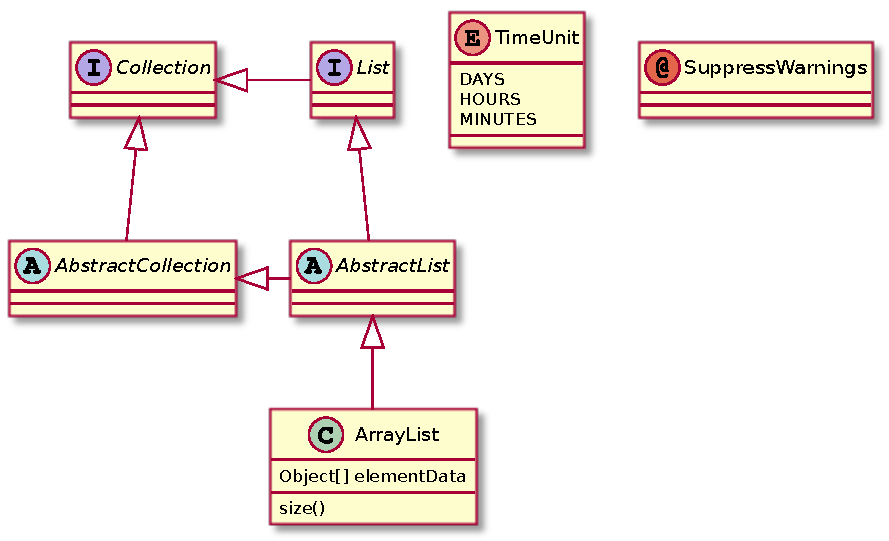
\includegraphics[width=0.5\linewidth]{figures/classes.pdf}
	\caption{A class diagram created with PlantUML}
	\label{fig:classes}
\end{figure}

You may want to reference images in your thesis.
%
In this case, you are encouraged to make them \emph{floating}, and reference them by means of labels.
%
For instance, in \Cref{fig:classes}, we describe a class diagram produced by means of \href{http://plantuml.com}{PlantUML}.

%----------------------------------------------------------------------------------------
\chapter{Implementation} % possible chapter for Projects
\label{chap:implementation}
%----------------------------------------------------------------------------------------

Write implementation here.

\lstinputlisting[
	float,
	language=Java,
	caption={My very first program in Java},
	label={lst:helloworld},
]{listings/HelloWorld.java}

You may need to reference listings in your thesis.
%
In this case, you are encouraged to make them \emph{floating}, and reference them by means of labels.
%
For instance, in \Cref{lst:helloworld}, we describe an hello world program in Java.

%----------------------------------------------------------------------------------------
\chapter{Validation} % possible chapter for Projects
\label{chap:validation}
%----------------------------------------------------------------------------------------

Write implementation here

%----------------------------------------------------------------------------------------
\chapter{\conclusionsname}
\label{chap:conclusions}
%----------------------------------------------------------------------------------------

Write conclusions here.


%----------------------------------------------------------------------------------------
% BIBLIOGRAPHY
%----------------------------------------------------------------------------------------

%\nocite{*} % uncomment this to show all the reference in the .bib file
\bibliographystyle{plain}
\bibliography{bibliography}


\end{document}